\documentclass[a4paper]{article}
% \documentclass[a4paper]{ctexart}

\usepackage{amssymb}
\usepackage{amsmath}
\usepackage{CJKutf8}
\usepackage{color}
\usepackage{enumerate}
\usepackage{fancyhdr}
\usepackage{geometry}
\usepackage{graphicx}
\usepackage{indentfirst}
\usepackage{latexsym}
\usepackage{mathrsfs}
\usepackage{subfigure}
\usepackage{textcomp}
% \usepackage{unicode-math}

\usepackage{amsthm}
\usepackage{algorithm}
\usepackage{algorithmic}

\usepackage{flafter}
\usepackage{booktabs, longtable}
\usepackage{pxfonts}
\usepackage{cite}

% \usepackage[colorlinks,linkcolor=red]{hyperref}

\newcommand{\avg}[1]{\left\langle #1 \right\rangle}
\newcommand{\cProj}{{\mathcal{P}}}
\newcommand{\cProjLH}{{\mathscr{P}}}
\newcommand{\curve}[1]{\widetilde{#1}}
\newcommand{\dif}{\mathrm{d}}
\newcommand{\dt}{\tau}
\newcommand{\Dim}{{\textsc{D}}}
\newcommand{\DRLN}[1]{{\cal D}_{\curve{#1}}}
\newcommand{\ebold}{{\mathbf{e}}}
\newcommand{\ibold}{{\mathbf{i}}}
\newcommand{\jbold}{{\mathbf{j}}}
\newcommand{\nPoly}{N_{\kappa}^{\Dim}}

\newcommand{\Div}{{\mathbf{D}}}
\newcommand{\Grad}{{\mathbf{G}}}
\newcommand{\Proj}{{\mathbb{P}}}
\newcommand{\Lapl}{{\mathbf{L}}}
\newcommand{\MARS}{{\mathfrak L}_{\mathrm{Mars}}}
\newcommand{\Zero}{\hat{0}}
\newcommand{\One}{\hat{1}}
\newcommand{\Int}{\mathrm{int}}
% \newcommand{\ShowRevised}[1]{{\color{red} #1}}
\newcommand{\ShowRevised}[1]{#1}

% \setmainfont{Latin Modern Roman}
% \setsansfont{Latin Modern Sans}
% \setmonofont{Latin Modern Mono}
% \setmathfont{Latin Modern Math}

\DeclareMathAlphabet{\mathcal}{OMS}{cmsy}{m}{n}
\let\mathbb\relax % remove the definition by unicode-math
\DeclareMathAlphabet{\mathbb}{U}{msb}{m}{n}

\begin{document}
% \begin{CJK*}{UTF8}{gbsn}
\begin{CJK*}{UTF8}{gkai}
  \CJKindent
  % ------------中文设置--------------------------
  \makeatletter %将文献引用作为上标出现,增加括号,
  \def\@cite#1#2{\textsuperscript{[{#1\if@tempswa , #2\fi}]}}
  \makeatother
  \newtheorem{theorem}{{定理}}
  \newtheorem{proposition}[theorem]{{命题}}
  \newtheorem{lemma}[theorem]{{引理}}
  \newtheorem{corollary}[theorem]{{推论}}
  \newtheorem{definition}[theorem]{{定义}}
  \newtheorem{question}[theorem]{{问题}}

  \renewcommand{\refname}{\centerline{参考文献}}
  \renewcommand{\tablename}{表}
  % \renewcommand{\captionlabeldelim}{\quad}
  % ===================Image settings========================%
  \renewcommand{\figurename}{图}
  \renewcommand{\abstractname}{摘要}
  % \renewcommand{\captionlabeldelim}{\quad} %Need caption2 macro package
  % ===============End image settings========================%
  % -----------中文设置--------------------------
  
  \title{Numerical Simulation of COVID-19 in Brazil}
  \author{李阳 \, 11935018}
  \date{\today}

  \maketitle

  % \begin{abstract}

  %   \setlength{\parindent}{0pt}
  %   \setlength{\parskip}{1.5ex plus 0.5ex minus 0.2ex} %\noindent

  % \end{abstract}


  % \textbf{关键字}:

  % \clearpage

  \pagestyle{fancy}
  \fancyhead{}
  \lhead{李阳}
  \chead{}
  \rhead{Numerical Simulation of COVID-19 in Brazil}

  \section{引言}
  在本报告中,
  我们将对巴西新冠肺炎数据(表\ref{fig:numbers})进行简单数值模拟,
  最后再简要介绍下经典的动力学传染病数学模型:SIR模型。
  在以下的2、3两节中,
  我们将分别采用两种最基本的数值分析方法:
  插值和拟合。由于目前巴西疫情形式还较为严峻,
  累计确诊数据仍然呈现出较快上升趋势,
  在插值时我们就选用三次样条函数,
  而在拟合时选择三次多项式。
  在第4节中,
  我们回顾SIR模型。
  \begin{table}[H]
    \centering
    \begin{tabular}[H]{|c|c|c|c|c|c|c|c|c|c|c|}
      \hline
      日期 & 3.30 & 4.07 & 4.15 & 4.23 & 5.01 & 5.09 & 5.17 & 5.25 & 6.02 & 6.10 \\
      \hline
      数据 & 4256 & 12341 & 25758 & 46348 & 87187 & 147003 & 233511 & 363211 & 526447 & 707412 \\
      \hline
    \end{tabular}
    \caption{巴西疫情累计确诊人数统计}
    \label{fig:numbers}
  \end{table}

  \section{三次样条插值}
  对给定数据点$(x_i, y_i), 1\le i\le n$,
  三次样条插值函数$S(x)$满足
  \begin{displaymath}
    S(x_i)=y_i, \quad 1\le i \le n, \quad S(x)|_{[x_i, x_{i+1}]}\in\mathbb{P}_3, \quad 1\le i\le n-1, \quad S(x)\in\mathcal{C}^2[x_1, x_n],
  \end{displaymath}
  这里我们假定$x_i$是按递增顺序给定。
  为了使得三次样条插值函数唯一,
  我们还需要提适当的边界条件,
  在这里我们考虑非节点(not-a-knot)三次样条插值:
  \begin{displaymath}
    s'''(x) \text{在}x=x_2 \text{ 和} x=x_{n-1}\text{处存在}.
  \end{displaymath}
  对于具体的三次样条函数求解过程
  (求解某三对角线性方程组从而得到在$[x_i, x_{i+1}]$上表达式),
  我们在此不再赘述,
  我们直接使用\verb|matlab|提供的\verb|spline|函数。
  对于数据点,
  我们以3月30日作为时间基点,
  对于$y_i$我们都除以1000处理。
  代码见附录,
  最终得到的数值结果如图\ref{fig:spline}。
  \begin{figure}
    \centering
    \subfigure[巴西新冠肺炎数据的三次样条插值]{
      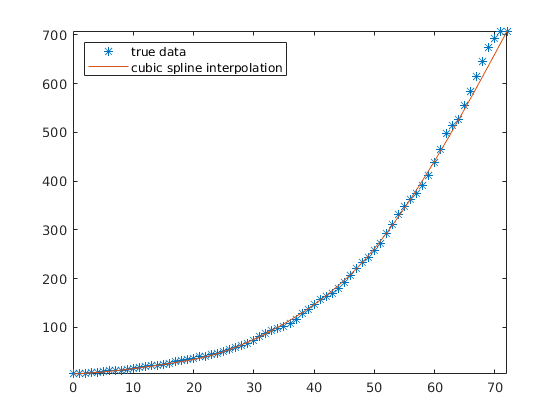
\includegraphics[width=0.43\linewidth]{png/spline.png}
      \label{fig:spline}}
    \hfill
    \subfigure[巴西新冠肺炎数据的最小二乘拟合]{
      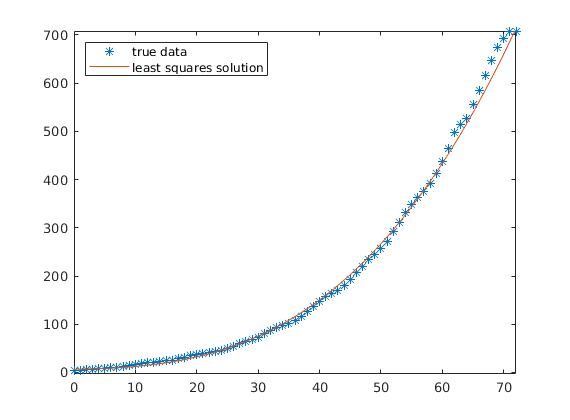
\includegraphics[width=0.43\linewidth]{png/leastSquares.png}
      \label{fig:fitting}
    }
    \label{fig:data}
    \caption{巴西新冠肺炎数据的插值与拟合}
  \end{figure}
  我们可以看到得到的三次样条曲线与真实数据是比较吻合的。


  \section{最小二乘拟合}
  对于给定数据点$(x_i, y_i), (1\le i\le n)$,
  最小二乘拟合归结为寻求$p(x)=\sum_{j=0}^na_jx^j$使得$p$最小化
  \begin{displaymath}
    \min_{q\in\mathbb{P}_n}\sum_{i=1}^n|p(x_i)-y_i|^2.
  \end{displaymath}
  对于该问题,
  我们可采用QR分解来做,
  具体过程在此就不再赘述,
  在\verb|matlab|中直接使用左除就可以求解。
  最终得到的拟合多项式为
  \begin{displaymath}
    p_3(x) = 6.6933 + 0.1910x + 0.0243x^2+0.0015x^3,
  \end{displaymath}
  数值结果见图\ref{fig:fitting}.

  \section{SIR模型}
  SIR模型是在传染病学研究中较为经典的模型,
  其将人群分为易感人群(Susceptible)、感染人群(Infected)以及恢复
  (Recovered)人群,数量分别记为$S(t), I(t)$以及$R(t)$,
  并做如下假设:
  \begin{itemize}
  \item
    人口数量始终不变(不考虑人口的出生、死亡和流动等种群动力因素),
    即
    \begin{displaymath}
      N(t) = S(t) + I(t) + R(t) = N, \quad \forall t\ge 0.
    \end{displaymath}
  \item
    一个感染人一旦与易感者接触就会具有一定的传染力,
    假设该传染概率为$\beta$,
    易感人数减少的速度等于转变为感染人数的速度,
    即
    \begin{displaymath}
      \frac{\dif S(t)}{\dif t} = -\beta \frac{I(t)}{N(t)}S(t).
    \end{displaymath}
  \item
    单位时间内从感染者中恢复的人数与感染者数量成正比,
    以$\gamma$来表示从感染到恢复的比例,
    从而
    \begin{displaymath}
      \frac{\dif R(t)}{\dif t} = \gamma I(t)
    \end{displaymath}
  \end{itemize}
  基于以上这三个假设,
  我们还可以得到感染人数增加的速度等于易感者增加的速度减去恢复人数增加的速度,
  即
  \begin{displaymath}
    \frac{\dif I(t)}{\dif t} = \beta \frac{I(t)}{N(t)}S(t) - \gamma I(t).
  \end{displaymath}
  总结以上假设以及结论,
  我们得到如下常微分方程组
  \begin{align*}
    \frac{\dif S(t)}{\dif t} &= -\beta \frac{I(t)}{N(t)}S(t) \\
    \frac{\dif I(t)}{\dif t} &= \beta \frac{I(t)}{N(t)}S(t)-\gamma I(t) \\
    \frac{\dif R(t)}{\dif t} &= \gamma I(t),
  \end{align*}
  初始条件为
  \begin{displaymath}
    S(0) = S_0, I(0) = I_0, R(0) = 0,
  \end{displaymath}
  根据假设, 其中$S_0$和$I_0$应当满足
  \begin{displaymath}
    S_0 + I_0 = N.
  \end{displaymath}
  对于该ODE,我们可采用\verb|matlab|提供的ODE求解器进行求解,
  例如\verb|ode45|和\verb|ode23s|等等,
  代码见附录,以下是我们得到的数值结果。($N=2000, \beta=0.08, \gamma=0.04,
  I_0=20, S_0=N-I_0=1980$)
  \begin{figure}[H]
    \centering
    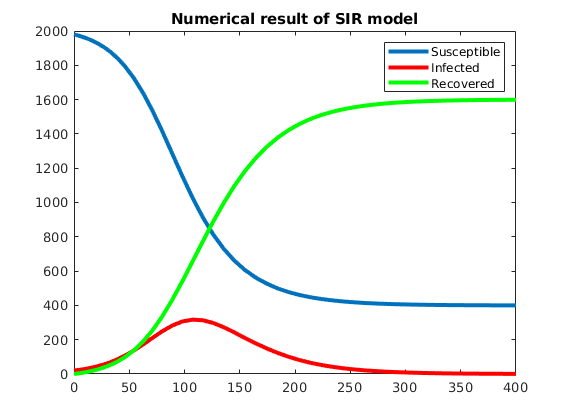
\includegraphics[scale=0.60]{png/SIR.png}
    \caption{SIR模型数值模拟结果}
  \end{figure}
  从该结果我们可以看到疾病最终将得到控制。

  对于现实情况的数值模拟,该模型还是远远不够的,
  我们还需要考虑很多因素,
  例如$\beta, \gamma$都可能都是变系数的,
  上述的三条假设在实际政策的影响下甚至也有可能是完全不对的。
  所以我们还得考虑对该模型进行某些修改,
  例如加入某些随机参数,
  对最终得到的数学模型还得使用更深入的数学理论才能求解,
  对这些因素的考量应该都已经超出了本报告的范围。

  \section{附录}
  在本节中我们附上生成该报告中图片的所有代码。
  三次样条插值代码:
\begin{verbatim}
% true data
xx = linspace(0,72,73)';
yy = [4256;4681;5861;7011;8165;9216;10431;11298;
    12341;14152;16238;18176;19943;21042;22625;23955;
    25758;29015;30891;34485;36925;39144;40814;43592;
    46348;50512;54043;59479;63328;67446;73235;80246;
    87187;92630;96559;101826;108620;116299;127389;137309;
    147003;156604;163510;170021;179457;192081;206507;220291;
    233511;244052;257396;271885;291579;310087;330890;347398;
    363211;374898;391222;411821;438238;465166;498440;514849;
    526447;555383;584016;614941;646006;673587;691758;707412;
    707412]/1000;
plot(xx,yy,'*')
axis([0 72 4.2 708])
hold on
% data points for interpolation
x = linspace(0,72,10)';
y = [4256; 12341; 25758; 46348; 87187; 147003;
    233511; 363211; 526447; 707412]/1000;
u = linspace(0,72)'; % for plotting
% Perform cubic spline interpolation
v = spline(x,y,u);
plot(u,v,'-')
hold off
legend('true data', 'cubic spline interpolation', 'Location', 'NorthWest')
\end{verbatim}
  最小二乘拟合代码:
\begin{verbatim}
% true data
xx = linspace(0,72,73)';
yy = [4256;4681;5861;7011;8165;9216;10431;11298;
    12341;14152;16238;18176;19943;21042;22625;23955;
    25758;29015;30891;34485;36925;39144;40814;43592;
    46348;50512;54043;59479;63328;67446;73235;80246;
    87187;92630;96559;101826;108620;116299;127389;137309;
    147003;156604;163510;170021;179457;192081;206507;220291;
    233511;244052;257396;271885;291579;310087;330890;347398;
    363211;374898;391222;411821;438238;465166;498440;514849;
    526447;555383;584016;614941;646006;673587;691758;707412;
    707412]/1000;
plot(xx,yy,'*')
axis([0 72 -3.2 708])
hold on
x = linspace(0,72,10)';
y = [4256; 12341; 25758; 46348; 87187; 147003;
    233511; 363211; 526447; 707412]/1000;
A = [x.^0 x.^1 x.^2 x.^3];
a = A\y;
u = linspace(0,72)';
plot(u,a(1)+a(2)*u+a(3)*u.^2+a(4)*u.^3,'-')
hold off
legend('data points','least squares solution','Location','NorthWest')
\end{verbatim}

  SIR模型数值模拟代码:
\begin{verbatim}
N = 2000; % total population
beta = 0.08; gamma = 0.04; 
SIRfunc = @(t, y) [ -beta*y(2)/N*y(1);
    beta*y(2)/N*y(1)-gamma*y(2);
    gamma*y(2)];
t0 = 0; tfinal = 400;
% initial conditions
I0 = 20; S0 = N-I0; R0 = 0;
y0 = [S0; I0; R0];
[t, y] = ode45(SIRfunc,[t0,tfinal],y0);
plot(t,y(:,1),'-',t,y(:,2),'r-',t,y(:,3),'g-','LineWidth',3);
legend('Susceptible','Infected','Recovered')
title('Numerical result of SIR model')
\end{verbatim}

  % {\footnotesize
  % \bibliographystyle{abbrv}
  % \bibliography{bib/Reference}
  % }

\end{CJK*}
\end{document}

%%% Local Variables:
%%% mode: latex
%%% TeX-master: t
%%% End:
